\chapter{Sistemi di trasmissione in modulazione numerica}
Un sistema di trasmissione di bit generati da una sorgente digitale può utilizzare un canale trasmissivo passa banda applicando le tecniche di modulazione analogica alle forme d'onda che codificano i simboli “0” e “1” in banda base. \`{E} necessario adattare tali segnali alla funzione di trasferimento del canale passa banda: lo spettro rettangolare di una forma d'onda di Nyquist con $\delta=0$ e banda $B$ viene modulato per rientrare nelle frequenze della banda passante del canale.

Al ricevitore è necessario operare inversamente: demodulare il segnale passa banda per riportarlo in banda base, per ottenere le forme d'onda ad intersimbolo nullo, campionare con stringenti requisiti di precisione dell'estrattore del timing e applicare il decisore per ricostruire la sequenza di bit trasmessa. 

\begin{figure}[!ht]
	\centering
	\resizebox{\textwidth}{!}{
	\begin{tikzpicture}[>=latex',fitted/.style={draw,thick,dotted,inner sep=4mm,rounded corners}]
	\coordinate(c0);
	\node[block,right=1.5cm of c0](b0){GFO};
	\node[mult,right=1cm of b0](m0){}edge[<-](b0);
	\node[below=1cm of m0](t0){$\cos{\omega t}$}edge[->](m0);
	\node[block,right=1cm of m0](b1){MT}edge[<-](m0);
	\node[sum,right=1cm of b1](s0){$+$}edge[<-](b1);
	\node[above=1cm of s0](n0){$n(t)$}edge[->](s0);
%	\node[mult,right=1cm of s0](m1){}edge[<-](s0);
%	\node[below=1cm of m1](t1){$2 \cos{\omega t}$}edge[->](m1);
	\node[block,right=1cm of s0](b2){FR}edge[<-](s0);
	\node[block,right=1cm of b2](b3){DEM}edge[<-](b2);
	\node[block,right=1cm of b3](b4){$H_R$}edge[<-](b3);
	\node[campionatore,right=1cm of b4](q0){}edge[<-](b4);
	\node[block,right=1cm of q0](b5){DEC}edge[<-](q0);
	\coordinate[right=1.5cm of b5](c1);
	\draw[->](c0)--node[above,near start]{bit}(b0);
	\draw[->](b5)--node[above,near end]{bit}(c1);
	\node[fitted, fit=(b0)(m0),label=above:Trasmettitore]{};
	\node[fitted, fit=(b2)(b3)(b4)(b5),label=above:Ricevitore]{};
	\node[fitted, fit=(b1)(s0),label=above:Canale]{};
	\end{tikzpicture}
	}
	\caption{Schema di trasmissione in modulazione numerica}
\end{figure}

Tutto quanto studiato nel capitolo \ref{cap:sis_telcom_band_pass} sui sistemi di telecomunicazione su canale radio passa banda, con riferimento alle modulazioni d'ampiezza e angolare di segnali analogici, si può applicare alla trasmissione numerica.

\section{Amplitude Shift Keying}
La modulazione d'ampiezza in un mezzo trasmissivo passa banda modifica l'ampiezza della portante trasmessa in accordo con la forma d'onda da trasmettere. Un semplice esempio di modulazione \ac{ASK} si ottiene modulando una portante sinusoidale con una forma d'onda a codifica di linea ortogonale, costituita da rettangoli di ampiezza positiva unitaria per codificare il simbolo “1” e forma d'onda nulla per codificare lo “0” (fig.~\ref{fig:OOK_modulazione}). Tale modulazione del tipo “tutto o niente” \ac{OOK} può essere realizzata con un interruttore che pone a massa l'uscita di un oscillatore che genera la sinusoide portante quando si deve trasmettere il simbolo “0” (fig.~\ref{fig:OOK_circuito}).

Per un migliore sfruttamento della potenza trasmessa si utilizza la codifica antipodale che modula la portante con valori costanti positivi o negativi. Si realizza di fatto una modulazione 2-\ac{PSK} in cui la forma d'onda ha inviluppo costante e la portante inverte la fase ogni volta che il segnale modulante cambia segno (fig.~\ref{fig:2PSK_modulazione}).

Nel caso la portante sia modulata da forme d'onda con inviluppo non costante si parla propriamente di modulazione \ac{ASK} (fig.~\ref{fig:ASK_modulazione}).

\begin{figure}[ht]\centering
	\def\omegazero{2*pi*4}
	\subfloat[Modulazione \acf{OOK}]{
		\begin{tikzpicture}
		\begin{axis}[enlargelimits,yscale=0.6,xlabel=$t$,ylabel=$s_T(t)$,xtick=\empty,ytick={-1,1},black,samples=300]
		\addplot[domain=0:1] {sin((\omegazero*x))};
		\addplot[domain=2:4] {sin((\omegazero*x))};
		\addplot[thick,domain=0:4.1] {rect(x,0,1)+rect(x,2,4)};
		\end{axis}
		\end{tikzpicture}\label{fig:OOK_modulazione}
	}\quad\subfloat[Circuito \ac{OOK}]{
	\begin{circuitikz}
	\coordinate(c0);
	\coordinate[above=1cm of c0] (c1);
	\coordinate[below=1cm of c0] (c2);
	\coordinate[right=2cm of c0] (c3);
	\coordinate[above=.25cm of c3] (c4);
	\coordinate[below=.25cm of c3] (c5);
	\coordinate[right=of c3] (c6);
	\draw(c1)to[vco,l=$\sen{\omega_0 t}$]++(2,0);
	\draw[-o](c1)++(2,0)-|(c4);
	\draw(c2)node[ground]{}(c2);
	\draw[-o](c2)-|(c5);
	\draw[o-](c3)--node[above]{$1$}node[below]{$0$}(c6);
	\end{circuitikz}\label{fig:OOK_circuito}
	}\quad\subfloat[Modulazione ad inviluppo costante (2-\ac{PSK})]{
	\begin{tikzpicture}
	\begin{axis}[enlargelimits,yscale=0.6,xlabel=$t$,ylabel=$s_T(t)$,xtick=\empty,ytick={-1,1},black,samples=300]
	\addplot[domain=0:1] {sin((\omegazero*x))};
	\addplot[domain=1:2] {sin((\omegazero*x+pi))};
	\addplot[domain=2:3] {sin((\omegazero*x))};
	\addplot[domain=3:4] {sin((\omegazero*x+pi))};
	\addplot[thick,domain=0:4.1] {rect(x,0,1)-rect(x,1,2)+rect(x,2,3)-rect(x,3,4)};
	\end{axis}
	\end{tikzpicture}\label{fig:2PSK_modulazione}
	}\quad\subfloat[Circuito 2-\ac{PSK}]{
	\begin{circuitikz}
	\coordinate(c0);
	\coordinate[above=1cm of c0] (c1);
	\coordinate[below=1cm of c0] (c2);
	\coordinate[right=2cm of c0] (c3);
	\coordinate[above=.2cm of c3] (c4);
	\coordinate[below=.2cm of c3] (c5);
	\coordinate[right=of c3] (c6);
	\draw(c1)to[vco,l=$\sen{\omega_0 t+\pi}$]++(2,0);
	\draw[-o](c1)++(2,0)-|(c4);
	\draw(c2)to[vco,l=$\sen{\omega_0 t}$]++(2,0);
	\draw[-o](c2)++(2,0)-|(c5);
	\draw[o-](c3)--node[above]{$1$}node[below]{$0$}(c6);
	\end{circuitikz}\label{fig:2PSK_circuito}
	}\quad\subfloat[Modulazione ad inviluppo non costante (\ac{ASK})]{
	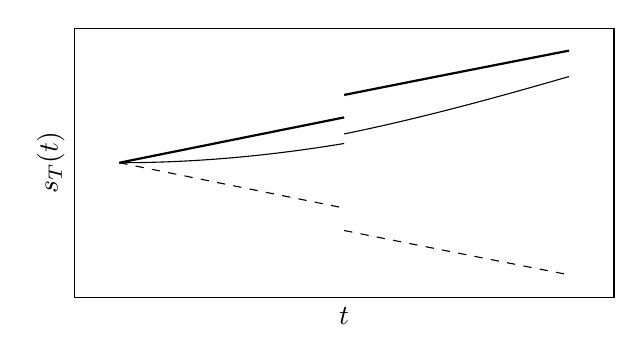
\begin{tikzpicture}
	\begin{axis}[enlargelimits,yscale=0.6,xlabel=$t$,ylabel=$s_T(t)$,xtick=\empty,ytick={-1,1},black,samples=300]
	\addplot[domain=0:1] {sin((\omegazero*x))*sin((2*pi*x))};
	\addplot[thick,domain=0:1] {sin((2*pi*x))};
	\addplot[domain=0:1,dashed] {-sin((2*pi*x))};
	\addplot[domain=1:2] {sin((\omegazero*x))*sin((2*pi*x+pi))};
	\addplot[thick,domain=1:2] {sin((2*pi*x+pi))};
	\addplot[domain=1:2,dashed] {-sin((2*pi*x+pi))};
	\end{axis}
	\end{tikzpicture}\label{fig:ASK_modulazione}
	}\quad\subfloat[Circuito \ac{ASK}]{
	\begin{circuitikz}
		\coordinate(c0);
		\coordinate[above=1cm of c0] (c1);
		\coordinate[below=1cm of c0] (c2);
		\node[mult,right=2cm of c0] (c3){};
		\coordinate[right=of c3] (c4);
		\draw(c1)to[vco,l=$\sen{\omega_0 t+b_m\cdot\pi}$]++(2,0)-|(c3);
		\draw(c2)to[vco,l=$\sen{\omega_0 t}$]++(2,0)-|(c3);
		\draw(c3)--(c4);
	\end{circuitikz}
}
\caption{Modulazione numerica \acf{ASK}}
\end{figure}

\section{Quadrature Amplitude Modulation}
Per aumentare l'efficienza spettrale di un sistema di trasmissione numerica in modulazione di ampiezza \ac{ASK} si sfruttano le due bande laterali per trasmettere due segnali modulanti con portanti in quadratura, ad esempio dei bit pari sul canale in fase e dei bit dispari sul canale in quadratura. 

Nella trasmissione analogica in \ac{DSB-SC} l'imperfetta ortogonalità delle portanti causata da un errore di fase nella modulazione in quadratura genera un accoppiamento tra i canali. La trasmissione numerica è più robusta all'interferenza tra canali finché è garantita una buona discriminazione dei livelli associati ai simboli in ricezione. L'operazione di decisione al ricevitore consiste nella verifica del sottospazio nel quale cade il punto identificato dalle misure ottenute dai due campionatori sul canale in fase e sul canale in quadratura.

Dati due segnali digitali in codifica antipodale di ampiezza $\pm a$ modulanti la portante in fase $\cos{\omega_0 t}$ e la portante in quadratura $\sen{\omega_0 t}$ si ottengono, utilizzando le formule trigonometriche: \[\sen{\alpha}=\cos{\alpha-\frac{\pi}{2}}\quad-\cos{\alpha}=\cos{\pi-\alpha}\] \[\Cos\alpha+\Cos\beta=2\cos{\frac{\alpha+\beta}{2}}\cos{\frac{\alpha-\beta}{2}}\qquad\Cos\alpha-\Cos\beta=-2\sen{\frac{\alpha+\beta}{2}}\sen{\frac{\alpha-\beta}{2}}\]
\begin{description}
	\footnotesize
	\item[Bit “11”] Portante in fase $c^\text{I}=+a$, portante in quadratura $c^\text{Q}=+a$:
	\[\begin{split}a\cos{\omega_0 t}+a\sen{\omega_0 t}&=a\cos{\omega_0 t}+a\cos{\omega_0 t-\frac{\pi}{2}}=2a\cos{\omega_0 t-\frac{\pi}{4}}\cos{\frac{\pi}{4}}=\sqrt{2}a\cos{\omega_0 t-\frac{\pi}{4}}\end{split}\]
	\item[Bit “10”] Portante in fase $c^\text{I}=+a$, portante in quadratura $c^\text{Q}=-a$:
	\[\begin{split}a\cos{\omega_0 t}-a\sen{\omega_0 t}&=a\cos{\omega_0 t}-a\cos{\omega_0 t-\frac{\pi}{2}}=-2a\sen{\omega_0 t-\frac{\pi}{4}}\sen{\frac{\pi}{4}}=\sqrt{2}a\cos{\omega_0 t-\frac{3}{4}\pi}\end{split}\]
	\item[Bit “00”] Portante in fase $c^\text{I}=-a$, portante in quadratura $c^\text{Q}=-a$:
	\[\begin{split}-a\cos{\omega_0 t}-a\sen{\omega_0 t}&=a\cos{\pi-\omega_0 t}-a\cos{\omega_0 t-\frac{\pi}{2}}=2a\sen{\omega_0 t-\frac{3}{4}\pi}\sen{\frac{\pi}{4}}=\sqrt{2}a\cos{\omega_0 t-\frac{5}{4}\pi}\end{split}\]
	\item[Bit “01”] Portante in fase $c^\text{I}=-a$, portante in quadratura $c^\text{Q}=+a$:
	\[\begin{split}-a\cos{\omega_0 t}+a\sen{\omega_0 t}&=-a\cos{\omega_0 t}+a\cos{\omega_0 t-\frac{\pi}{2}}=-2a\sen{\omega_0 t-\frac{\pi}{4}}\sen{\frac{\pi}{4}}=\sqrt{2}a\cos{\omega_0 t-\frac{7}{4}\pi}\end{split}\]	
\end{description}

\begin{figure}[ht]
\centering
\subfloat[Rappresentazione fasoriale portanti]{
	\begin{tikzpicture}[>=latex']
	\def\anglealpha{30}
	\def\anglebeta{\anglealpha-90}
	\def\anglegamma{\anglealpha-45}
	\def\angletheta{\anglealpha-135}
	\coordinate (b11) at (\anglegamma:1.414cm);
	\coordinate (b01) at (\angletheta:1.414cm);
	\coordinate (b00) at (\anglegamma:-1.414cm);
	\coordinate (b10) at (\angletheta:-1.414cm);
	\draw[->] (-1.5,0)--(1.6,0);
	\draw[->] (0,-1.5)--(0,1.6);
	\draw[gray](0,0) circle [radius=1.41cm];
	\filldraw[fill=gray!20,draw=gray!50!black] (0,0) -- (5mm,0mm) arc [start angle=0, end angle=\anglealpha, radius=5mm] -- cycle node[right]{\footnotesize$\omega_0 t$};
	\draw[dotted](\anglealpha:1.41cm)node{\footnotesize$\cos{\omega_0 t}$}--(0,0)--(\anglebeta:1.41cm)node{\footnotesize$\sen{\omega_0 t}$};
	\draw[thick] (b11) circle(2pt) node[below right]{$11$} --(0,0)--(b00) circle(2pt) node[above left]{$00$};
	\draw[thick](b01) circle(2pt) node[below left]{$01$}--(0,0)--(b10) circle(2pt) node[above right]{$
		10$};
	\draw[dashed](b11)--(b10)--(b00)--(b01)--cycle;
	\end{tikzpicture}}\quad%
\subfloat[Portanti modulate in quadratura]{
	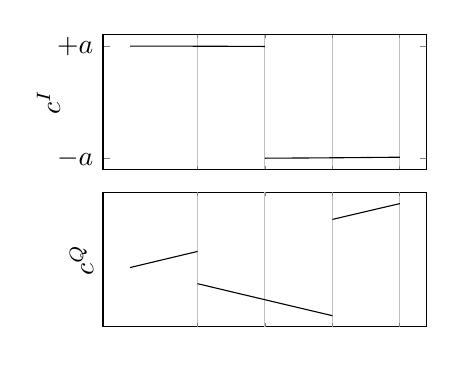
\begin{tikzpicture}
	\begin{axis}[yshift=2cm,xscale=.6,yscale=.3,smooth,xtick=\empty,enlargelimits,ytick={-1,1},yticklabels={$-a$,$+a$},ylabel=$c^\text{I}$,extra x ticks={3.14,6.28,9.42,12.56},extra x tick labels=\empty,extra x tick style={grid=major}]
		\addplot [domain=0:2*pi]{cos(x)};
		\addplot [domain=2*pi:4*pi]{-cos(x)};
	\end{axis}
	\begin{axis}[xscale=.6,yscale=.3,smooth,xtick=\empty,enlargelimits,ylabel=$c^\text{Q}$,ytick={-1,1},yticklabels={$-a$,$+a$},extra x ticks={3.14,6.28,9.42,12.56},extra x tick labels=\empty,extra x tick style={grid=major}]
		\addplot [domain=0:pi]{sin(x)};
		\addplot [domain=pi:3*pi]{-sin(x)};
		\addplot [domain=3*pi:4*pi]{sin(x)};
	\end{axis}
	\end{tikzpicture}}
\quad\subfloat[Segnale modulato 4-\ac{PSK}]{
	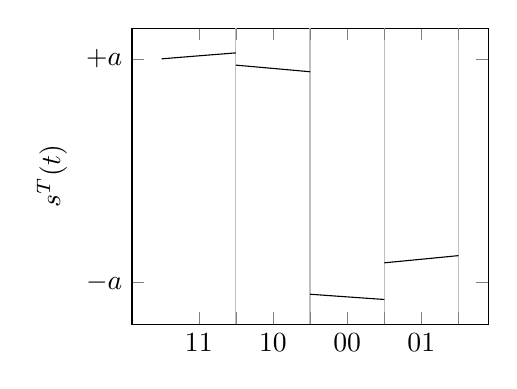
\begin{tikzpicture}
		\begin{axis}[scale=.66,smooth,ylabel=$s^\text{T}(t)$,xtick=\empty,ytick={-1,1},yticklabels={$-a$,$+a$},xtick={1.57,4.71,7.85,10.99},xticklabels={$11$,$10$,$00$,$01$},extra x ticks={3.14,6.28,9.42,12.56},extra x tick labels=\empty,extra x tick style={grid=major}]
		\addplot [domain=0:pi]{cos(x)+sin(x)};
		\addplot [domain=pi:2*pi]{cos(x)-sin(x)};
		\addplot [domain=2*pi:3*pi]{-cos(x)-sin(x)};
		\addplot [domain=3*pi:4*pi]{-cos(x)+sin(x)};
		\end{axis}
	\end{tikzpicture}}
	\caption{Modulazione di ampiezza con portanti in quadratura (4-\ac{PSK})}
\end{figure}

La modulazione \ac{QAM} con portanti in quadratura di forme d'onda rettangolari risulta in una modulazione 4-\ac{PSK} con una sinusoide scalata di una ampiezza costante, pulsazione $\omega_0 t$, e fasi con quattro possibili valori equidistribuiti sull'angolo giro, pari a $\ang{45}$, $\ang{135}$, $\ang{225}$, $\ang{315}$ a seconda della combinazione delle ampiezze antipodali. \`{E} possibile assegnare in modo arbitrario le sequenze di bit alle varie configurazione di fase ma si predilige la numerazione di Grey in base al criterio di distanza minima di Hamming di 1 bit tra simboli adiacenti.

Utilizzando segnali modulanti rettangolari multilivello si può estendere la modulazione \ac{QAM} mantenendo la stessa occupazione spettrale con modulazioni di fase 8-\ac{PSK} (3 bit per simbolo) o 16-\ac{PSK} (4 bit per simbolo). Il dimensionamento di un tale sistema è limitato dal rumore sul canale trasmissivo che introduce una deviazione di fase tale da causare una errata decisione sul valore di soglia al demodulatore per simboli adiacenti sulla circonferenza.

\subsection{Dimensionamento}
Nel dimensionamento di un sistema di trasmissione numerico \ac{QAM} con portanti in quadratura valgono le considerazioni relative ad un sistema con una sola portante con modulazione \ac{ASK} binario o \ac{PSK} applicate separatamente alle due portanti, per cui il decisore a soglia al ricevitore verifica il livello del segnale ricevuto a cui è sommato un disturbo che causa errore.

Nel seguente schema è rappresentato, in un sistema di assi cartesiani solidali alle portanti in quadratura, la costellazione dei valori assunti da una modulazione \ac{QAM} a valle del filtro di ricezione affetto da rumore, con la separazione in settori circolari del piano in corrispondenza delle soglie tra i livelli 
\begin{figure}[ht]
	\centering
	\begin{tikzpicture}[>=latex']
	\draw[->](-1.5,0)--(2.1,0)node[right]{\footnotesize$\sen{\omega_0 t}$};
	\draw[->](0,-1.5)--(0,1.8)node[above]{\footnotesize$\cos{\omega_0 t}$};
	\draw[gray](0,0)circle[radius=1.41cm];
	\foreach\anglealpha/\bits/\shade in {0/000/50,45/001/25,90/011/50,135/010/25,180/110/50,225/111/25,270/101/50,315/100/25} {
		\pgfmathparse{\anglealpha-22.5}\def\anglebeta{\pgfmathresult}
		\pgfmathparse{\anglealpha+22.5}\def\angletheta{\pgfmathresult}
		\draw[fill=gray!50!black,draw=gray!50!black,dotted] (0,0) -- (2cm,0mm) arc [start angle=\anglebeta, end angle=\angletheta, radius=2cm] -- cycle;
		\draw(\anglealpha:1.41cm)decorate[decoration={random steps,segment length=3pt,amplitude=2pt}]{circle(10pt)} node{\footnotesize$\bits$};
	}
	\end{tikzpicture}
	\caption{Schema spazio dei segnali nella modulazione 8-\ac{PSK}}
\end{figure}

Il ricevitore per decidere quale sia la configurazione ricevuta verifica in quale sottospazio ricadono le due misure ottenute dai due campionatori sul canale in fase e in quadratura applicando un criterio di distanza minima.

Al ricevitore le componenti indipendenti del rumore in fase $n^\text{I}(t)$ e quadratura $n^\text{Q}(t)$ si sommano ai segnali rettangolari antipodale ricevuti attenuati:

\[\begin{array}{ll}
11\colon\begin{cases}
+a\stackrel{I}{\longrightarrow}+k\cdot a+n^\text{I} \\
+a\stackrel{Q}{\longrightarrow}+k\cdot a+n^\text{Q}
\end{cases} &
10\colon\begin{cases}
+a\stackrel{I}{\longrightarrow}+k\cdot a+n^\text{I} \\
-a\stackrel{Q}{\longrightarrow}-k\cdot a+n^\text{Q}
\end{cases} \\\\
00\colon\begin{cases}
-a\stackrel{I}{\longrightarrow}-k\cdot a+n^\text{I} \\
-a\stackrel{Q}{\longrightarrow}-k\cdot a+n^\text{Q}
\end{cases}	&
01\colon\begin{cases}
-a\stackrel{I}{\longrightarrow}-k\cdot a+n^\text{I} \\
+a\stackrel{Q}{\longrightarrow}+k\cdot a+n^\text{Q}
\end{cases}
\end{array}\]

Il rumore passa banda sovrapposto alle portanti in quadratura rappresenta una variabile aleatoria gaussiana bidimensionale a simmetria circolare, ovvero un vettore con ampiezza e fase casuale (fig.~\ref{fig:var_aleatoria_gaussiana_bidimensionale}).

\begin{figure}[ht]\centering\def\amp{2.0}\def\var{0.5}
	\subfloat{
		\begin{tikzpicture}
		\begin{axis}[xlabel=$v^\text{I}$,ylabel=$v^\text{Q}$,small,domain=-6:6,domain y=-6:6,colormap name=graywhite]
		\addplot3[surf,z buffer=auto,faceted color=black,samples=32]{
			\amp/\var*exp(-((x-3)^2+(y-3)^2)/(2*\var))+
			\amp/\var*exp(-((x+3)^2+(y-3)^2)/(2*\var))+
			\amp/\var*exp(-((x-3)^2+(y+3)^2)/(2*\var))+
			\amp/\var*exp(-((x+3)^2+(y+3)^2)/(2*\var))};
		\end{axis}
		\end{tikzpicture}}\quad\def\amp{2.0}\def\var{0.5}
	\subfloat{
		\begin{tikzpicture}
		\begin{axis}[view={30}{60},xlabel=$v^\text{I}$,ylabel=$v^\text{Q}$,small,domain=-6:6,domain y=-6:6,colormap name=graywhite]
		\addplot3[surf,faceted color=black,z buffer=auto,samples=32] {
			\amp/\var*exp(-((x-4.24)^2+y^2)/(2*\var))+
			\amp/\var*exp(-((x-3)^2+(y-3)^2)/(2*\var))+
			\amp/\var*exp(-((x-3)^2+(y+3)^2)/(2*\var))+
			\amp/\var*exp(-(x^2+(y-4.24)^2)/(2*\var))+
			\amp/\var*exp(-(x^2+(y+4.24)^2)/(2*\var))+
			\amp/\var*exp(-((x+4.24)^2+y^2)/(2*\var))+
			\amp/\var*exp(-((x+3)^2+(y-3)^2)/(2*\var))+
			\amp/\var*exp(-((x+3)^2+(y+3)^2)/(2*\var))};
		\end{axis}
		\end{tikzpicture}}
	\caption{Rappresentazione delle densità di probabilità del segnale in ricezione modulato affetto da rumore espresso da variabile aleatoria gaussiana bidimensionale}
	\label{fig:var_aleatoria_gaussiana_bidimensionale}
\end{figure}

La probabilità di errore è valutabile come il volume della densità di probabilità condizionata esterna all'area delimitata dai valori di soglia tra simboli contigui.
\[p(\epsilon)=\sum_{i=0}^{M-1}p(\epsilon|s_i)p(s_i)=\frac{1}{M}\sum_{i=0}^{M-1}p(\epsilon|s_i)\]
\[p(\epsilon|s_i)=p(s_j^R|s_i^T)=p(0_R|1_T\vee 1_R|0_T)\quad i\neq j\]

Tale probabilità si può valutare estraendo il sistema binario equivalente ottenuto valutando il rapporto tra la distanza tra i vertici di due vettori contigui della costellazione \ac{QAM}:
\begin{equation}
p(\epsilon)=\f{Q}{\frac{d}{2\sigma_n}}
\end{equation}

Tale approssimazione per un sistema multilivello M-\ac{PSK} è lecita in quanto è possibile trascurare la probabilità di errore di confondere un livello con livelli più lontani di quelli contigui, ovvero i settori circolari in cui è diviso il piano.

Per un sistema di trasmissione numerico M-\ac{PSK} con codifica di Grey la probabilità di errore su un bit è pari alla probabilità di confondere il livello con i due adiacenti ovvero il doppio di quella del sistema binario equivalente:
\begin{equation}
\text{BER}=2\f{Q}{\frac{d}{2\sigma_n}}
\label{eq:qam_mpsk_biterrorrate}
\end{equation}

Essendo la potenza del rumore una caratteristica del mezzo trasmissivo e degli apparati di ricezione a parità di potenza della portante aumentare il numero di livelli fa diminuire la distanza tra i vertici della costellazione con la sovrapposizione delle code delle gaussiane, aumentando la probabilità di errore su bit.

Data una rumorosità del sistema se si vuole aumentare la velocità di trasmissione aumentando il numero di livelli rappresentati per ogni trasmissione di un simbolo, mantendo costante il \keyword{BER}, è necessario incrementare la potenza di trasmissione per mantenere la distanza tra i vertici dei vettori contigui. 
Tale sistema risulta inefficiente in termini di potenza oltre la modulazione 16-\ac{PSK} risultando inutilizzato lo spazio all'interno del cerchio ove giacciono i vertici della costellazione M-\ac{PSK}.

A tal fine si introduce la modulazione di ampiezza multilivello M-\ac{QAM} con portanti in quadratura e inviluppo non costante: la costellazione dei vertici è disposta a reticolo imponendo la distanza minima tra vertici contigui tale da mantenere costante la probabilità d'errore. Ad esempio la 4-\ac{QAM} risulta in due portanti in quadratura modulate da segnali a due livelli. Nel caso 16-\ac{QAM} con 4 livelli per portante si hanno segnali trasmessi secondo la costellazione in fig.~\ref{fig:16-QAM} con un $\text{BER}=4\f{Q}{\frac{d}{2\sigma_n}}$. Raddoppiando ancora i livelli su entrambe le portanti si ottengono $M=4^4=256$ configurazioni. 

Per ottimizzare ulteriormente il valore valore di picco di potenza dell'amplificatore in corrispondenza delle configurazioni ai vertici del quadrato si spostano tali configurazioni nei punti med\^{i} dei lati, mantenendo regolare il passo tra i punti del reticolo come in fig.~\ref{fig:256-QAM}. Altre tecniche di riempimento ottimizzano ulteriormente lo spazio tra i punti in modo che siano equidistanti al prezzo di una maggiore complessità.

\begin{figure}[ht]
	\centering
	\subfloat[16-\ac{QAM}]{
	\begin{tikzpicture}[>=latex']
	\draw[->](-2.5,0)--(2.6,0)node[right]{\footnotesize$\sen{\omega_0 t}$};
	\draw[->](0,-2.5)--(0,2.6)node[above]{\footnotesize$\cos{\omega_0 t}$};
	\draw[gray!50](0,0)circle[radius=2.25cm];
	\draw[->](0,0)--(1.5,1.5);
	\draw[dotted](-.5,.5)--(.5,.5)--node[below]{$d$}(1.5,.5)(.5,-.5)--(.5,1.5);
	\foreach \cx in {-1.5,...,1.5}
		\foreach \cy in {-1.5,...,1.5}
		{
			\draw (\cx,\cy) circle (2mm);
			\fill (\cx,\cy) circle (1mm);
		}
	\end{tikzpicture}\label{fig:16-QAM}}%
	\quad\subfloat[256-\ac{QAM}]{
		\begin{tikzpicture}[>=latex']
		\draw[->](-2.7,0)--(2.9,0)node[right]{\footnotesize$\sen{\omega_0 t}$};
		\draw[->](0,-2.7)--(0,2.9)node[above]{\footnotesize$\cos{\omega_0 t}$};
		\draw[gray!50](0,0)circle[radius=2.6cm]; %r=2.55+0.05
		\draw[gray!80,->](0,0)--(59:2.55cm);
		\newdimen\bailout
% 		creo un quadrato di lato 2R 
% 		in cui visualizzare x punti interni alla circonferenza di raggio R
%		x : 4*R^2 = 256 : pi*R^2
%		lato = 51 mm  spazio tra i punti 3mm   18 punti per lato
		\foreach \cx in {-2.55,-2.25,...,2.85}  % 18
		\foreach \cy in {-2.55,-2.25,...,2.85}  % 18
		{
			\pgfmathparse{\cx*\cx+\cy*\cy}
			\bailout = \pgfmathresult cm
			\ifdim \bailout < 7.29 cm % (0.3*18/2)^2
				\draw (\cx,\cy) circle (1mm);
				\fill (\cx,\cy) circle (0.5mm);
			\fi
		}
		\end{tikzpicture}\label{fig:256-QAM}}
	\caption{Schema spazio dei segnali nella modulazione M-\ac{QAM} a 16 e 256 configurazioni}
\end{figure}

\subsection{Vantaggi dell'inviluppo costante}
Nella modulazione \ac{PSK} la forma d'onda è a inviluppo costante: l'informazione è contenuta alla fase della portante pertanto è possibile mandare in saturazione gli amplificatori di trasmissione per il massimo guadagno di potenza. La sinusoide della portante viene squadrata e assume al limite la forma di un'onda quadra alla stessa frequenza della portante modulata, conservando gli istanti di attraversamento dello zero al cambio di segno. Se il segnale modulante è un treno di impulsi rettangolari all'uscita dell'amplificatore in saturazione si ottiene un segnale con spettro costituito dalle repliche dei seni cardinali centrati nelle armoniche della frequenza portante (fig.~\ref{fig:portante_squadrata_PSK}). \`{E} possibile limitare in banda lo spettro eliminando le code del $\sinc{f}$ mediante filtro passa banda, in quanto in ricezione si devono fornire forme d'onda ad intersimbolo nullo con termini spettrali contenuti all'interno del lobo principale. Maggiore attenzione è necessaria per segnali modulanti di ampiezza generica su portante squadrata: il segnale ricostruito viene distorto dalle non linearità. La portante squadrata filtrata passa-banda presenta spigoli smussati quindi un inviluppo non costante, amplificando e filtrando in ricezione si ottiene un segnale con modulazione di fase spuria.

\begin{figure}[ht!]\centering
	\begin{tikzpicture}          
	\begin{axis}[xlabel=$f$,ylabel=$H(f)$,xtick={20,25,30},xticklabels={$f_0$,$2 f_0$,$3 f_0$},axis x discontinuity=crunch,xtickmin=20,ytick={1},yscale=.66,samples=500,domain=15:35]
	\addplot[gray] {(sinc(x-20,1)+sinc(x-25,1)+sinc(x-30,1)+sinc(x-40,1))^1.1};
	\addplot[black,thick,domain=19:21] {(sinc(x-20,1)+sinc(x-25,1)+sinc(x-30,1))};
	\addplot[gray,dashed] {rect(x,19,21)};
	\end{axis}                   
	\end{tikzpicture}
	\caption{Spettro portante modulata \ac{PSK} all'ingresso e all'uscita di un amplificatore spinto in saturazione}
	\label{fig:portante_squadrata_PSK}
\end{figure}

\subsection{Offset temporale tra canali in quadratura}
Confrontando le densità spettrali di potenza generate da diversi sistemi di trasmissione in modulazione numerica, a parità di prestazioni, si preferisce il segnale con la minore occupazione di banda sul mezzo trasmissivo.

Nelle modulazioni di fase \ac{PSK} sono le brusche variazioni di fase che incrementano l'occupazione spettrale del segnale. Per il \ac{PSK} binario sono gli indispensabili salti di fase di $\pi$, per il M-\ac{PSK} si ha il salto di fase massimo sempre di $\pi$ per configurazioni opposte.

Per ridurre la banda necessaria in trasmissione si introduce la modulazione in quadratura con offset temporale O-\ac{QAM}.
I simboli della sequenza numerica generati con una frequenza di cifra $f_s$ vengono inviati sul canale in quadratura con un ritardo di mezzo periodo di cifra $T_s/2$ rispetto al canale in fase: in tal modo non si può verificare una transizione contemporanea di polarità sulle due portanti, per cui la loro somma potrà differire al massimo di $\ang{90}$. Riducendo l'ampiezza delle discontinuità sfasando temporalmente le commutazioni si dimezza l'occupazione in banda.

\clearpage
\section{Frequency Shift Keying \ac{FSK}}
La modulazione di frequenza \ac{FSK} è una tecnica di modulazione per la trasmissione numerica digitale. Le forme d'onda trasmesse per codificare i simboli “0” e “1” sono sinusoidi a frequenze $f_0$ e $f_1$. Il generatore di forme d'onda nel modulatore \ac{FSK} può essere realizzato con due oscillatori alle frequenze $f_0$ o $f_1$ e uno switch commutatore comandato che seleziona la forma d'onda in base al bit da trasmettere (fig.~\ref{fig:FSK_modulatore_oscillatori}). In alternativa è possibile utilizzare un oscillatore controllato in tensione con in ingresso la forma d'onda rettangolare rappresentante i bit da trasmettere (fig.~\ref{fig:FSK_modulatore_VCO}).

La prima soluzione nella transizione tra oscillazioni a frequenze diverse si può presentare discontinuità nel segnale, data la difficoltà di commutare esattamente in corrispondenza degli zeri, introducendo componenti spettrali non legate all'informazione ma che causano una maggiore occupazione di banda.
Con un oscillatore controllato in tensione la variazione di frequenza nell'anello in retroazione varia con continuità, e  a meno di un transitorio in cui la forma d'onda risulta distorta sono assenti salti di tensione e componenti spettrali spurie.
Le due tecniche di realizzazione del modulatore \ac{FSK} portano oltre che ad una diversa occupazione di banda anche a diverse soluzioni in demodulazione.



\begin{figure}[!ht]
\centering\subfloat[\ac{GFO} con due oscillatori]{
\begin{tikzpicture}
\node[block](f0){$f_0$};
\coordinate[below=5mm of f0] (c0);
\coordinate[right=2cm of c0] (c1);
\coordinate[above=2mm of c1] (c2);
\coordinate[below=2mm of c1] (c3);
\coordinate[right=15mm of c1] (c4);
\node[block, below=5mm of c0](f1){$f_1$};
%\node[clock, below=1cm of c4](clk){}edge[->](c4);
\draw[-o](f0)-|(c2);
\draw[-o](f1)-|(c3);
\draw[o-](c1)--(c4);
\node[clock,below=5mm of c4](clk){};
\draw[decorate,decoration=snake](c1)+(2mm,5mm) -- +(12mm,5mm);
\draw[decorate,decoration={snake,segment length=5}](c1)+(2mm,-5mm) -- +(12mm,-5mm);
\end{tikzpicture}\label{fig:FSK_modulatore_oscillatori}}\quad\subfloat[\ac{GFO} con oscillatore controllato]{
\begin{tikzpicture}
\node[block](b0){$VCO$};
\coordinate[left=1cm of b0](c0){};
\node[clock,left=5mm of c0](clk){}edge[->](c0);
\coordinate[right=1cm of b0](c1);
\draw[-](b0)--(c1);
\draw[o-](c0)--node[above]{$0$}node[below]{$1$}(b0);
\draw[decorate,decoration=snake](c1)+(-5mm,5mm) -- +(5mm,5mm);
\draw[decorate,decoration={snake,segment length=5}](c1)+(-5mm,-5mm) -- +(5mm,-5mm);
\end{tikzpicture}\label{fig:FSK_modulatore_VCO}}
\caption{Modulatore \ac{FSK}}
\end{figure}

Il ricevitore è costituito da un circuito \keyword{demodulatore} molto semplice che non richiede il recupero di una \keyword{portante}. Un demodulatore incoerente si realizza confrontando l'uscita di due filtri passabanda adattati alle forme d'onda trasmesse centrati alle frequenze $f_0$ e $f_1$. Il decisore può così ricostruire la forma d'onda rettangolare in banda base che rappresenta la sequenza di simboli trasmessa.

\begin{figure}[!ht]\centering
\begin{tikzpicture}[>=latex',fitted/.style={draw,thick,dotted,inner sep=4mm,rounded corners}]
\node[passabanda,label=below:$f_0$](f0){};
\node[block, right=1cm of f0](i0){Rilevatore inviluppo} edge[<-](f0);
\coordinate[below=8mm of f0] (c2);
\coordinate[left=1.5cm of c2] (c1);
\coordinate[left=1.5cm of c1] (c0);
\draw[decorate,decoration=snake](c0)+(-5mm,5mm) -- +(5mm,5mm);
\draw[decorate,decoration={snake,segment length=5}](c0)+(-5mm,-5mm) -- +(5mm,-5mm);
\node[passabanda,label=below:$f_1$,below=8mm of c2](f1){};
\node[block, right=1cm of f1](i1){Rilevatore inviluppo}edge[<-](f1);
\node[block, right=55mm of c2](cc){Decisore $\gtrless$};
\coordinate[right=2cm of cc] (c3);
\draw[->](c0)--(c1)|-(f0);
\draw[->](c0)--(c1)|-(f1);
\draw[->](i0)-|(cc);
\draw[->](i1)-|(cc);
\draw[->](cc)--node[above]{$0/1$}(c3);
\node[fitted, fit=(c1)(f0)(f1)(i0)(i1)(cc),label=above:Demodulatore incoerente \ac{FSK}]{};
\end{tikzpicture}
\caption{Schema demodulatore incoerente \ac{FSK}}
\end{figure}

\clearpage
\section{Continuous Phase \ac{FSK}}
La codifica di linea della modulazione \ac{FSK} non trasmette forme d'onda in codifica antipodale il che causa una perdita di efficienza rispetto alla codifica antipodale della modulazione \ac{PSK} di almeno $\SI{3}{\decibel}$. Le discontinuità nella fase della portante della modulazione \ac{PSK} sono causa di inefficienza spettrale che è possibile superare con opportuni accorgimenti nella modulazione \ac{FSK}.

Al fine di ottenere una alta efficienza spettrale si definisce la modulazione \ac{CP-FSK} imponendo per costruzione l'ortogonalità delle forme d'onda trasmesse e la continuità di fase ad ogni periodo di simbolo $T$.

L'ortogonalità impone che le frequenze adottate per la trasmissione dei simboli “0” e “1” non possano essere svincolate dal tempo di simbolo, il periodo $T$, dovendo far rientrare un numero intero di oscillazioni nel periodo, e non possono essere svincolate tra loro, dovendo imporre ad ogni tempo di simbolo la continuità di fase del segnale.

\begin{figure}[ht!]\centering
\def\freqA{20}
\foreach\freqB[count=\c] in{40,45,50} {
\subfloat[$T=\frac{1}{10},f_0=\SI{\freqA}{\hertz},f_1=\SI{\freqB}{\hertz}$]{
 	\begin{tikzpicture}
 	\begin{axis}[xlabel=$f$,ylabel=$H_s(f)$,xtick={\freqA,\freqB},xticklabels={$f_0$,$f_1$},axis x discontinuity=crunch,xtickmin=10,ytick={1},yscale=.5,samples=500,domain=5:60]
 	\addplot[black] {sinc(x-\freqA,1)+sinc(x-\freqB,1)};
 	\addplot[red!50,densely dotted] {sinc(x-\freqA,1)};
 	\addplot[blue!50,densely dotted] {sinc(x-\freqB,1)};
 	\end{axis}
% 	\begin{scope}[xshift=-5cm]
% 	\begin{axis}[scale=.5,domain=0:.1,samples=256,ytick={-1,1},xtick={.1},xticklabels={$T$},xlabel=$t$,ylabel=$s(t)$]
% 	\addplot[red!50] {cos(2*pi*\freqA*x)};
% 	\addplot[blue!50]{cos(2*pi*\freqB*x)};
% 	\addplot[thick,black]{cos(2*pi*\freqA*x)*cos(2*pi*\freqB*x)};
% 	\end{axis}
% 	\end{scope}
 	\end{tikzpicture}}}
\label{fig:FSK_ortogonali}
\end{figure}

L'\keyword{ortogonalità} dalle forme d'onda trasmesse ha inoltre l'effetto di ridurre la densità spettrale di potenza dei lobi secondari dei $\sinc{}$ compresi tra le frequenze $f_0$ e $f_1$ (notare la differenza tra fig.~\ref{fig:FSK_ortogonali}b e fig.~\ref{fig:FSK_ortogonali}c).

Si ha l'ortogonalità imponendo che:
\begin{equation}
\intd{0}{T}{\cos{2\pi f_0 t}\cos{2\pi f_1 t}}{t}=0
\label{eq:sin_ortogonali}
\end{equation}
dove
\[ \cos{2\pi f_0 t}\cos{2\pi f_1 t}=\frac{1}{2}\cos{2\pi(f_0+f_1)t}+\frac{1}{2}\cos{2\pi(f_1-f_0)t} \]
Risolvendo l'integrale \ref{eq:sin_ortogonali} si ha
\[ \frac{1}{2}\bound{0}{T}{\frac{\sin{2\pi(f_0+f_1)t}}{2\pi(f_0+f_1)}}+\frac{1}{2}\bound{0}{T}{\frac{\sin{2\pi(f_1-f_0)t}}{2\pi(f_1-f_0)}}=0\]
dove i termini si annullano per
\[ f_0+f_1=\frac{n}{2 T} \qquad f_1-f_0=\frac{m}{2 T} \]

L'ortogonalità richiesta da \ac{CP-FSK} è garantita dall'integrale nullo quando $f_0$ e $f_1$ sono multipli interi differenti di $\frac{1}{2 T}$. Per \ac{FSK} è sufficiente che siano multipli interi differenti di $\frac{1}{T}$.

\section{Minimum Shift Keying \ac{MSK}}
Tra le possibili scelte consentite dalla modulazione \ac{CP-FSK} quella che garantisce la minima occupazione di banda si ha imponendo la minima differenza tra le frequenze $f_0=\frac{n}{2T}$ e $f_1=\frac{n+1}{2T}$ pari a $f_1-f_0=\frac{1}{2T}$.
Per tali frequenze i lobi principali della densità spettrale di potenza hanno distanza minima (fig.~\ref{fig:FSK_ortogonali}a).

La portante modulata assume la seguente espressione:
\begin{equation}
s_T(t)=\sum_{m}{\cos{2\pi f_P t + b_m\frac{2\pi}{4T}t}\rect{\frac{t-m T}{T}}}
\label{eq:FSK_portante_modulata}
\end{equation}
dove la frequenza della portante è $f_P=(f_0+f_1)/2$ e il coefficiente $b_m$ codifica i bit di informazione secondo la convenzione:
\[ b_m=\begin{cases}
+1 & \text{“1”}\\-1 & \text{“0”}
\end{cases} \]

Tale espressione garantisce l'ortogonalità tra le forme d'onda ma non soddisfa la continuità di fase della portante, perché la sinusoide a frequenza $f_1=f_0+\frac{1}{2T}$ ha mezzo periodo in più rispetto a quella a frequenza $f_0$, come in fig.~\ref{fig:FSK_forme_d'onda}.

\begin{figure}[ht]\centering
\def\freqP{1}
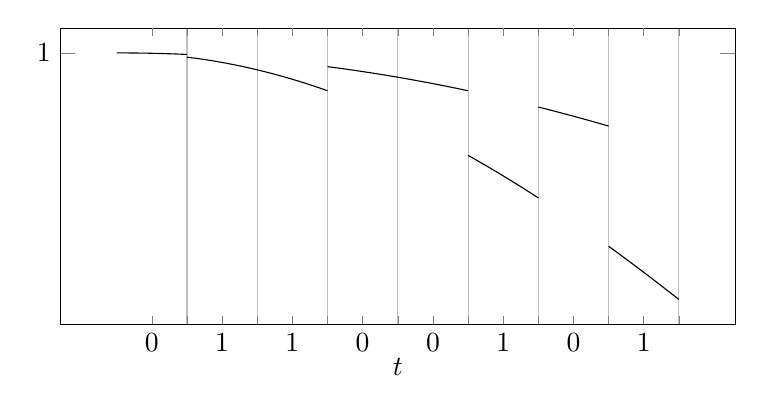
\begin{tikzpicture}
\begin{axis}[domain=0:8,samples=200,xscale=1.25,yscale=.66,xlabel=$t$,xtick={1,...,8},xticklabels=\empty,ytick={-1,1},xmajorgrids,extra x ticks={.5,1.5,2.5,3.5,4.5,5.5,6.5,7.5},extra x tick labels={0,1,1,0,0,1,0,1},extra x tick style={grid=none}]
\addplot[black,domain=0:1]{cos(2*pi*\freqP*x-pi*x/2)};
\addplot[black,domain=1:2]{cos(2*pi*\freqP*x+pi*x/2)};
\addplot[black,domain=2:3]{cos(2*pi*\freqP*x+pi*x/2)};
\addplot[black,domain=3:4]{cos(2*pi*\freqP*x-pi*x/2)};
\addplot[black,domain=4:5]{cos(2*pi*\freqP*x-pi*x/2)};
\addplot[black,domain=5:6]{cos(2*pi*\freqP*x+pi*x/2)};
\addplot[black,domain=6:7]{cos(2*pi*\freqP*x-pi*x/2)};
\addplot[black,domain=7:8]{cos(2*pi*\freqP*x+pi*x/2)};
\end{axis}
\end{tikzpicture}
\caption{Forme d'onda \ac{MSK}}
\label{fig:FSK_forme_d'onda}
\end{figure}

\`{E} possibile ottenere una codifica CP-\ac{MSK} eliminando le discontinuità di fase imponendo in presenza dei salti di fase il cambio del segno della forma d'onda, ovvero aggiungendo un contributo di fase pari a $\pi$. Tale modo di procedere non modifica l'informazione trasmessa in quanto tale informazione è legata alla frequenza e non alla fase della portante. Si modifica l'espressione della portante eq.~\ref{eq:FSK_portante_modulata} iniettando il contributo di fase $\phi_m$ che assume valore $0$ o $\pi$ tale da impedire i salti di fase (fig.~\ref{fig:FSK_forme_d'onda_fase_continua}):
\begin{equation}
s_T(t)=\sum_{m}{\cos{2\pi f_P t + b_m\frac{2\pi}{4T}t + \phi_m}\rect{\frac{t-m T}{T}}}
\label{eq:FSK_portante_modulata_fase_continua}
\end{equation}

Si ottiene così l'ortogonalità e la continuità di fase con il minimo valore di deviazione della frequenza, da cui il nome di modulazione CP-\ac{MSK} a spettro compatto.

\begin{figure}[ht]\centering
	\def\freqP{1}
	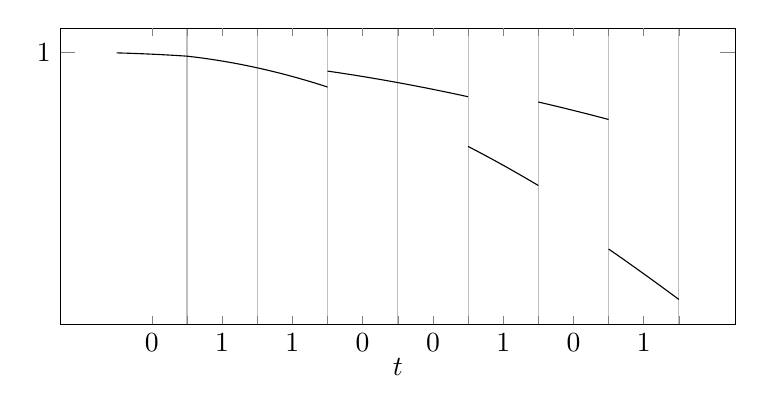
\begin{tikzpicture}
	\begin{axis}[domain=0:8,samples=200,xscale=1.25,yscale=.66,xlabel=$t$,xtick={1,...,8},xticklabels=\empty,ytick={-1,1},xmajorgrids,extra x ticks={.5,1.5,2.5,3.5,4.5,5.5,6.5,7.5},extra x tick labels={0,1,1,0,0,1,0,1},extra x tick style={grid=none}]
	\addplot[black,domain=0:1]{cos(2*pi*\freqP*x-pi*x/2+pi)};
	\addplot[black,domain=1:2]{cos(2*pi*\freqP*x+pi*x/2)};
	\addplot[black,domain=2:3]{cos(2*pi*\freqP*x+pi*x/2)};
	\addplot[black,domain=3:4]{cos(2*pi*\freqP*x-pi*x/2+pi)};
	\addplot[black,domain=4:5]{cos(2*pi*\freqP*x-pi*x/2+pi)};
	\addplot[black,domain=5:6]{cos(2*pi*\freqP*x+pi*x/2)};
	\addplot[black,domain=6:7]{cos(2*pi*\freqP*x-pi*x/2)};
	\addplot[black,domain=7:8]{cos(2*pi*\freqP*x+pi*x/2+pi)};
	\end{axis}
	\end{tikzpicture}
	\caption{Forme d'onda \ac{MSK} con continuità di fase}
	\label{fig:FSK_forme_d'onda_fase_continua}
\end{figure}

La modulazione \ac{M-FSK} è l'estensione a più livelli della modulazione \ac{FSK} con la trasmissione su $M$ portanti ortogonali. Un banco di filtri in ricezione farà passare solo un segnale alla frequenza trasmessa individuando il livello corrispondente e la configurazione di bit associata.

\begin{figure}[!ht]\centering
	\begin{tikzpicture}[scale=0.8,>=latex',fitted/.style={draw,thick,dotted,inner sep=4mm,rounded corners}]
	\node[passabanda,label=below:$f_0$](f0){};
	\node[block, right=1cm of f0](i0){Rilevatore inviluppo}edge[<-](f0);
	\node[mult,left=1cm of f0](p0){}edge[->](f0);
	\node[below=7mm of p0](m0){$2\cos{\omega_0 t}$}edge[<-](p0);
	\coordinate[below=1cm of p0] (c2);
	\coordinate[left=1cm of c2] (c1);
	\coordinate[left=15mm of c1] (c0);
	\draw[decorate,decoration=snake](c0)+(-5mm,5mm) -- +(5mm,5mm);
	\draw[decorate,decoration={snake,segment length=5}](c0)+(-5mm,-5mm) -- +(5mm,-5mm);
	\node[mult,below=1cm of c2](p1){};
	\node[passabanda,label=below:$f_1$,right=1cm of p1](f1){}edge[<-](p1);
	\node[below=7mm of p1](m1){$2\cos{\omega_1 t}$}edge[<-](p1);
	\node[block, right=1cm of f1](i1){Rilevatore inviluppo}edge[<-](f1);
	\node[block, right=75mm of c2](cc){Decisore $\gtrless$};
	\coordinate[right=15mm of cc] (c3);
	\draw[->](c0)--(c1)|-(p0);
	\draw[->](c0)--(c1)|-(p1);
	\draw[->](i0)-|(cc);
	\draw[->](i1)-|(cc);
	\draw[->](cc)--node[above]{$0/1$}(c3);
	\node[fitted, fit=(c1)(f0)(f1)(i0)(i1)(cc)(m0)(m1),label=above:Demodulatore coerente \ac{FSK}]{};
	\end{tikzpicture}
	\caption{Schema demodulatore coerente \ac{FSK}}
\end{figure}

Una ulteriore estensione consente la trasmissione in parallelo su $M$ portanti ortogonali ciascuna modulata \ac{QAM}. Ogni canale dello spettro ha il suo rapporto \ac{SNR} a seconda del quale si sceglie la migliore modulazione M-\ac{QAM}. Adattando la modulazione al rapporto segnale rumore variabile nel tempo si ottiene la modulazione \ac{OFDM} utilizzata nelle comunicazioni Wi-Fi e \ac{ADSL}.

\section{Demodulazione coerente}
L'utilizzo di portanti in quadratura nella modulazione \ac{QAM} e nella necessità di rilevare la fase nella modulazione \ac{PSK} richiede in ricezione una demodulazione coerente: è necessaria una oscillazione sincrona con la portante di riferimento per la fase locale al ricevitore. Tale informazione deve essere estratta direttamente dal segnale ricevuto.

Non è possibile pensare di filtrare ad esempio un segnale in modulazione \ac{PSK} binaria $\cos{\omega_0 t+a_i\pi}$ ($a_i=0$ se trasmetto “0” e $a_i=1$ se trasmetto “1”) (fig.~\ref{fig:2PSK_modulazione}) con un filtro molto stretto centrato attorno alla frequenza $f_0$: un filtro a banda molto stretta media i valori del segnale nel tempo su intervalli temporali lunghi fornendo un risultato a media nulla.

Per estrarre un riferimento di fase dalla portante è possibile utilizzare due procedure: raddrizzare il segnale ricevuto, a onda intera o a semionda, per ottenere oscillazioni risonanti alla frequenza $2f_0$; effettuare la quadratura del segnale ottenendo $\cos[2]{2\pi f_0 t+a_i\pi}=\frac{1}{2}+\frac{1}{2}\cos{4\pi f_0 t+a_i 2\pi}$ ed isolare la sinusoide a frequenza $2f_0$. Tali procedure si iterano per modulazioni di fase multilivello M-\ac{PSK}. 

\begin{esempio}
Nella modulazione 4-\ac{PSK} si trasmette il segnale $\cos{\omega_0 t+a_i\frac{\pi}{4}}=\cos{\omega_0 t+\frac{\pi}{4}+b_i\frac{\pi}{2}}$ con $a_i=1,3,5,7$, $b_i=0,1,2,3$.

Effettuando la quadratura si ottengono sinusoidi a frequenza doppia e quadrupla della portante:
\[\begin{split}\cos[2]{\omega_0 t+\frac{\pi}{4}+b_i\frac{\pi}{2}}=\frac{1}{2}+\frac{1}{2}\cos{2\omega_0 t+\frac{\pi}{2}+b_i\pi} \\ \cos[2]{2\omega_0 t+\frac{\pi}{2}+b_i\pi}=\frac{1}{2}+\frac{1}{2}\cos{4\omega_0 t+\pi+2b_i\pi}\end{split}\]
Non è possibile risalire alla fase iniziale $b_i\frac{\pi}{2}+\frac{\pi}{4}$. $\square$
\end{esempio}

All'uscita del filtro è necessario quindi un divisore di frequenza che è possibile realizzare con un circuito flip-flop. Tale operazione rende indeterminata la fase del segnale M-\ac{PSK} che è un multiplo di $2\pi/M$, con il risultato di ricostruire la corretta sequenza di bit o la sequenza complementare. Per risolvere tale problema è possibile inviare delle configurazioni binarie note sia al trasmettitore che al ricevitore tali da poter verificare l'inversione di segno  nell'oscillazione locale e ottenere il corretto sincronismo.

\begin{figure}[!ht]
\centering
\subfloat[Segnale \ac{PSK} binario $\cos{\omega_0 t+a_i\pi}$]{
	\begin{tikzpicture}
	\begin{axis}[enlargelimits,yscale=0.5,xlabel=$t$,ylabel=$s_T(t)$,xtick={1},ytick={-1,1},xmajorgrids,black,samples=300]
	\addplot[domain=0:1] {sin((2*pi*3*x))};
	\addplot[domain=1:2] {sin((2*pi*3*x+pi))};
	\end{axis}
	\end{tikzpicture}}%
\quad%
\subfloat[Raddrizzamento ad onda intera]{
\begin{tikzpicture}
\begin{axis}[enlargelimits,yscale=0.5,xlabel=$t$,ylabel=$s_T(t)$,xtick={1},ytick={-1,1},xmajorgrids,black,samples=500]
\addplot[domain=0:2] {abs(sin((2*pi*3*x)))};
\end{axis}
\end{tikzpicture}
}

\subfloat[Raddrizzamento a semionda]{
	\begin{tikzpicture}
	\begin{axis}[enlargelimits,yscale=0.4,xlabel=$t$,ylabel=$s_T(t)$,xtick={1},ytick={-1,1},xmajorgrids,black,samples=300]
	\addplot[domain=0:1] {sin((2*pi*3*x))>0?sin((2*pi*3*x)):0};
	\addplot[domain=1:2] {sin((2*pi*3*x+pi))>0?sin((2*pi*3*x+pi)):0};
	\end{axis}
	\end{tikzpicture}}%
\quad%
\subfloat[Quadratura del segnale]{
	\begin{tikzpicture}
	\begin{axis}[enlargelimits,yscale=0.4,xlabel=$t$,ylabel=$s_T(t)$,xtick={1},ytick={0,1},xmajorgrids,black,samples=300]
	\addplot[domain=0:2] {(sin((2*pi*3*x)))^2};
	\end{axis}
	\end{tikzpicture}}
\caption{Estrazione della portante da segnale \ac{PSK} binario}
\end{figure}

\section{Modulazioni differenziali}
\`{E} possibile svincolarsi dalla necessità di estrarre la fase assoluta dalla portante mediante la codifica \ac{DPSK}: si associano i simboli “0” e “1” alle transizione di fase piuttosto che al valore assoluto della fase. Nel \ac{DPSK} binario in trasmissione si fa cambiare la fase della portante rispetto alla fase del periodo precedente per trasmettere “1”, si lascia invariata la fase per trasmettere “0”. Nella modulazione 4-\ac{DPSK} si lascia invariata la fase per trasmettere la coppia di bit “00” e si cambia la fase di multipli di $\pi/2$ per le successive configurazioni.

Per realizzare la modulazione \ac{DPSK} si può utilizzare il modulatore \ac{PSK} a patto di modificare la sequenza di binaria in ingresso, operando una complementazione del bit in funzione del bit inviato al modulatore nel periodo precedente, ottenibile con un circuito dotato di uno operatore logico XOR e un delay (fig.~\ref{fig:DPSK_circuiti}). Similmente in ricezione bisogna effettuare l'operazione duale ricostruendo la sequenza di bit di informazione, verificando la permanenza o la variazione della fase tra periodi successivi.
\begin{figure}[!ht]
	\centering
	\subfloat[Codificatore \ac{DPSK}]{
		\begin{circuitikz}[scale=.5, transform shape]
			\draw (0,1.5)node[american xor port](xor){}
			(xor.in 2)|-(-1.25,0) to[twoport,t=$\Delta T$] (0,0)-|(xor.out) to[short,-o]++(.5,0) (xor.in 1)to[short,-o]++(-.5,0);
		\end{circuitikz}}
		\quad\subfloat[Decodificatore \ac{DPSK}]{		
			\begin{circuitikz}[scale=.5, transform shape]
				\draw (0,0) node[american xor port](xor){}
				(xor.in 1)--++(-2,0)|- ++(0,-1.5)to[twoport,t=$\Delta T$]++(2,0)-|(xor.in 2) (xor.in 1)to[short,-o]++(-2.5,0) (xor.out)to[short,-o]++(.5,0);
			\end{circuitikz}}
			\caption{Circuiti per codifica e decodifica differenziale}
			\label{fig:DPSK_circuiti}
\end{figure}
Il vantaggio ottenuto con la codifica differenziale di non essere legata al valore assoluto della fase si paga in caso di errore su un bit al decisore: tale errore causa l'errata decodifica di un numero di bit almeno pari al numero di divisioni di frequenza.

\clearpage
\section{Esercizio dimensionamento ponte radio}
\begin{esercizio}
Si vuole dimensionare un ponte radio per la trasmissione numerica digitale alla velocità di $\SI{100}{\mega\bit\per\second}$ con una probabilità d'errore massima su bit pari a $p(\epsilon)=\num{e-7}$ su una distanza di $\SI{100}{\kilo\meter}$ e una probabilità di fuori servizio $p_\text{FS}=\num{e-3}$. Si consideri la possibilità di spezzare il collegamento in due tratte di $\SI{50}{\kilo\meter}$ per esigenze di visibilità.
\end{esercizio}

\begin{figure}[!ht]
	\centering
%	\resizebox{\textwidth}{!}{
		\begin{tikzpicture}[>=latex',fitted/.style={draw,thick,dotted,inner sep=4mm,rounded corners}]
		\coordinate(c0);
		\node[mult,right=1cm of c0](m0){};
		\node[below=1cm of m0](t0){$2\cos{\omega t}$}edge[->](m0);
		\node[passabasso,right=1cm of m0](b1){};
		\node[campionatore,right=1cm of b1](b2){};
		\node[decisore,right=1cm of b2](b3){};
		\coordinate[right=1.5cm of b3](c1);
		\draw[dot=A](c0)--(m0);
		\draw[dot=$\restrict{\frac{S}{N}}{\text{in}}$](m0)--(b1);
		\draw[dot=$\restrict{\frac{S}{N}}{\text{out}}$](b1)--(b2);
		\draw[dot=$\restrict{\frac{S}{N}}{\text{dec}}$](b2)--(b3);
		\draw[->](b3)--node[above,near end]{$p(\epsilon)$}(c1);
		\end{tikzpicture}
%	}
	\caption{Schema per il dimensionamento del ricevitore di sistema di trasm. numerica su ponte radio}
\end{figure}

Scopo del dimensionamento è determinare la potenza da impegnare in trasmissione per ottenere determinati rapporti segnale rumore nei diversi punti del sistema e rispettare i vincoli di progetto, quali la velocità di trasmissione nel numero di simboli o bit al secondo, la distanza da coprire, e i livelli minimi di qualità da garantire in ricezione quali la probabilità di errore su bit e la probabilità di fuori servizio.

Sono necessarie numerose ipotesi progettuali motivate dai vari aspetti dei fondamenti delle telecomunicazioni, che portano a scegliere il numero di tratte, la modulazione, la tipologia di codifica di linea, tenendo conto delle caratteristiche del mezzo trasmissivo.

\subsection{Risoluzione con singola tratta e modulazione \ac{PSK} binaria}
A partire dal requisito sulla probabilità di errore all'uscita del sistema, causata dal rumore termico gaussiano bianco, ipotizzando una codifica antipodale del segnale in modulazione \ac{PSK} binaria, resta individuato il rapporto segnale rumore al decisore pari a $\gamma^2$ (vedi eq.~\ref{eq:rapporto_segnale_rumore_uscita_filtro_adattato})
\[p(\epsilon)=\f{Q}{\gamma}=\f{Q}{\frac{2a}{2\sigma_n}}=\f{Q}{\frac{a}{\sigma_n}}=\num{e-7}\]
che corrisponde esprimendo in decibel $\restrict{\gamma^2}{\text{dB}}=10\Log\frac{a}{\sigma_n}=\SI{14.5}{\decibel}$.

Nell'ipotesi di modulazione \ac{PSK}, per la massima efficienza di amplificazione di potenza di forme d'onda rettangolari, si utilizzerà un filtro di ricezione non adattato, che causa una attenuazione per il fattore di forma di $\SI{0.5}{\decibel}$ (vedi cap.~\ref{cap:rinuncia_filtro_adattato}). 

Risalendo all'ingresso del filtro di ricezione si ottiene un rapporto segnale rumore pari a $\restrict{S/N}{\text{in}}=\frac{a^2}{h_n f_s/2}=\SI{15}{\decibel}$ essendo la potenza di picco del segnale, prima e dopo il demodulatore, pari al quadrato dell'ampiezza $a^2$. In ingresso al ricevitore prima del demodulatore si ha un segnale sinusoidale di potenza media, sia in fase che quadratura, pari a $P_R=a^2/2$.

La potenza del rumore è calcolata moltiplicando la banda monolatera $f_s/2$ per la densità spettrale di rumore, tenendo conto che la densità spettrale di rumore nella banda passante del mezzo trasmissivo dopo la demodulazione si somma in banda base risultando in $h_n=2 h'_n$, e da cui risulta
\[\restrict{\frac{S}{N}}{\text{A}}=\frac{a^2/2}{h_n f_s/2}=\frac{1}{2}\frac{a^2}{h_n f_s/2}=\frac{1}{2}\restrict{\frac{S}{N}}{\text{in}}=\SI{15}{\decibel}-\SI{3}{\decibel}=\SI{12}{\decibel}\]
con l'ipotesi di un fattore di rumore degli apparati pari a $F=\SI{10}{\decibel}$ la densità spettrale di rumore equivalente $h_n$ (ovvero rapportata alla banda monolatera $f_s/2$) è pari prima del campionatore a $F k T_0$, ovvero in decibel
\[h_n \frac{f_s}{2}=\underbrace{-174}_{k T_0}+\underbrace{10}_{F}+\underbrace{3}_{\cdot 2}+\underbrace{10\Log{50\cdot 10^6}}_{\frac{f_s}{2}}=\SI{-84}{\dBm}\]
Resta determinata così la potenza minima del segnale portante da garantire in ingresso al ricevitore che dovrà essere pari a $P_\text{R}=12-84=\SI{-72}{\dBm}$.

Si passa a dimensionare il trasmettitore per determinare la potenza della portante da trasmettere che sia sufficiente a maggiorare l'attenuazione del mezzo trasmissivo (cap.~\ref{cap:canale_radio_attenuazione_spazio_libero}) e l'attenuazione dovuta ai cammini multipli (cap.~\ref{cap:canale_radio_effetti_cammini_multipli}):
\[p_T=p_R+\alpha_\text{SL}+\alpha_\text{suppl}\]

L'attenuazione del mezzo trasmissivo è dovuta alla divergenza sferica del segnale radio nello spazio libero tra le antenne, ed è funzione della distanza e dall'area efficace delle antenne (eq.~\ref{eq:radio_attenuazione_spazio_libero}). Supponendo che le antenne in ricezione e trasmissione siano uguali, con un guadagno $G=\SI{30}{\decibel}$ alla frequenza di cifra $f_s=\SI{1}{\giga\hertz}$ (data dalla velocità di trasmissione), resta determinata l'area efficace dell'antenna (per eq.~\ref{eq:radio_legame_area_efficace_guadagno_antenna}) $A=\frac{G c^2}{4\pi f^2}=\SI{7.16}{\meter\squared}=\SI{8.5}{\decibel\meter\squared}$, per cui l'attenuazione di spazio libero:
\[\alpha_\text{SL}=10\Log(4\pi(\SI{100}{\kilo\meter})^2)-\restrict{G}{dB}-\restrict{A}{dB}=111-30-8.5=\SI{72.5}{\decibel}\]

Va considerata l'attenuazione supplementare causata dai cammini multipli in radiofrequenza che fanno giungere al ricevitore segnali con fasi incoerenti, risultando in una potenza di picco descrivibile da una variabile aleatoria esponenziale. La probabilità di fuori servizio $p_\text{FS}=\num{e-3}$, data come requisito del sistema, coincide con la probabilità che l'ampiezza del segnale risultante sia inferiore ad una soglia ovvero che la potenza picco-picco del segnale ricevuto sia inferiore alla potenza di fuori servizio $P_\text{FS}$. Troncando al primo termine la serie di Taylor si ottiene la relazione tra probabilità di fuori servizio e il margine di potenza per superare l'attenuazione supplementare
\[ p_\text{FS}=p(P_R^\text{PP}<\gamma)=1-\e{\frac{\gamma}{P_0}}\cong\frac{\gamma}{P_0}=\frac{1}{\alpha_\text{suppl}}\implies\alpha_\text{suppl}=\frac{1}{p_\text{FS}}=\SI{30}{\decibel}\]

Il sistema di trasmissione numerico digitale dimensionato per un ponte radio su singola tratta da 100 km richiede una potenza di trasmissione 
\[p_T=\SI{-72}{\dBm}+\SI{30}{\decibel}+\SI{72.5}{\decibel}=\SI{30.5}{\decibel}\]

\subsection{Risoluzione multitratta digitale}
\`{E} possibile realizzare lo stesso sistema di trasmissione sotto l'ipotesi di ponte radio multitratta digitale: si suddivide la distanza massima in più tratte in cascata, utilizzando apparecchiature intermedie che ricevono, amplificano e ritrasmettono il segnale da una tratta alla successiva, oppure di un sistema di rigenerazione numerico che ricostruito il segnale digitale lo ritrasmette alla tratta successiva. Nel secondo caso la probabilità d'errore dell'intero sistema si può approssimare con la probabilità d'errore della tratta maggiormente affetta da errore.
\[p_T(\epsilon)\cong p_S(\epsilon)\]

Il dimensionamento viene effettuato nell'ipotesi che la probabilità d'errore del sistema sia imputabile alla tratta peggiore. Questo modello riprende il concetto del fuori servizio: la tratta fuori servizio mette fuori servizio l'intero sistema di trasmissione.

Il dimensionamento del sistema di ricezione della singola tratta non cambia al variare della lunghezza della tratta: per garantire una certa probabilità di errore su bit, data la rumorosità del sistema di ricezione e il tipo di codifica e modulazione, si deve sempre ricevere una potenza di ricezione minima di $P_R=\SI{-72}{\dBm}$.

Il dimensionamento del sistema di trasmissione considera una attenuazione di spazio libero su una tratta di 50km che risulta essere $1/4$ di quella da 100 km, pertanto  \[\alpha_\text{SL}=10\Log(4\pi R^2)-\restrict{G}{dB}-\restrict{A}{dB}=105-30-8.5=\SI{66.5}{\decibel}\]
mentre l'attenuazione supplementare cambia, non per una diversa statistica dei cammini multipli, ma perché è dimezzata la probabilità di fuori servizio sulla singola tratta (infatti considerando trascurabile la probabilità che siano fuori servizio più tratte si ha $p_{\text{FS}}=p_{\text{fs}1}(1-p_{\text{fs}2})+(1-p_{\text{fs}1})p_{\text{fs}2}=1-(1-p_{\text{fs}1})(1-p_{\text{fs}2})=p_{\text{fs}1}+p_{\text{fs}2}$),
avendo tratte uguali $p_{\text{fs}1}=p_{\text{fs}2}=p_{\text{FS}}/2$ per cui aumenta l'attenuazione supplementare $\alpha_\text{suppl}=\SI{33}{\decibel}$.

La potenza di trasmissione sulla singola tratta sarà
\[P_T=-72+66.5+33=\SI{27.5}{\decibel}\]
che consente di risparmiare $\SI{3}{\decibel}$ per tratta, con una potenza trasmessa complessiva inalterata.

\subsection{Risoluzione con modulazione 4-\ac{PSK}}
In alternativa è possibile dimezzare la frequenza di simbolo portandola da $\SI{100}{\mega\bit}$ a $\SI{50}{\mega\bit}$ adottando la modulazione 4-\ac{PSK} con la trasmissione e ricezione su due canali con portanti in quadratura.

\begin{figure}[!ht]\centering
	\begin{tikzpicture}[>=latex',fitted/.style={draw,thick,dotted,inner sep=4mm,rounded corners}]
	\node[passabanda,label=below:$f_0$](f0){};
	\node[mult,left=1cm of f0](p0){}edge[->](f0);
	\node[below=7mm of p0](m0){$2\cos{\omega_0 t}$}edge[->](p0);
	\node[campionatore,right=1cm of f0](q0){};
	\coordinate[below=1cm of p0] (c2);
	\coordinate[left=1cm of c2] (c1);
	\coordinate[left=15mm of c1] (c0);
	\node[mult,below=1cm of c2](p1){};
	\node[passabanda,label=below:$f_0$,right=1cm of p1](f1){}edge[<-](p1);
	\node[below=7mm of p1](m1){$2\sen{\omega_0 t}$}edge[->](p1);
	\node[campionatore,right=1cm of f1](q1){};
	\coordinate[right=10mm of q0] (c4);
	\coordinate[right=10mm of q1] (c5);
	\node[decisore, right=55mm of c2](cc){};
	\coordinate[right=15mm of cc] (c3);
	\draw[dot=$\restrict{\frac{S}{N}}{\text{in}}$](p0)--(f0);
	\draw[dot=$\restrict{\frac{S}{N}}{\text{in}}$](p1)--(f1);
	\draw[dot=$\restrict{\frac{S}{N}}{\text{out}}$](f0)--(q0);
	\draw[dot=$\restrict{\frac{S}{N}}{\text{out}}$](f1)--(q1);
	\draw[dot=$\restrict{\frac{S}{N}}{\text{dec}}$](q0)--(c4);
	\draw[dot=$\restrict{\frac{S}{N}}{\text{dec}}$](q1)--(c5);
	\draw[->](c0)--(c1)|-(p0);
	\draw[->](c0)--(c1)|-(p1);
	\draw[->](c4)-|(cc);
	\draw[->](c5)-|(cc);
	\draw[->](cc)--node[above]{$0/1$}(c3);
	\node[fitted, fit=(c1)(f0)(f1)(i0)(i1)(q0)(q1)(cc)(m0)(m1),label=above:Demodulatore coerente \ac{FSK}]{};
	\end{tikzpicture}
	\caption{Schema demodulatore coerente 4-\ac{PSK}}
\end{figure}

Data la probabilità di errore $p(\epsilon)=\f{Q}{\gamma}=\num{e-7}$ bisogna dimensionare la potenza di picco del segnale delle componenti in fase e quadratura in modo tale da distanziare dai $N=2$ simboli adiacenti (eq.~\ref{eq:qam_mpsk_biterrorrate}), 
\[p(\epsilon)=N\f{Q}{\frac{d}{2\sigma_n}}\]
Resta individuato così il rapporto segnale rumore al decisore è \[\restrict{\frac{S}{N}}{\text{dec}}=\gamma^2=10\Log{p(\epsilon)}+\Log N=\SI{14.5}{\decibel}+\SI{0.3}{\decibel}=\SI{14.8}{\decibel}\]
Il rapporto segnale rumore in ingresso al filtro di ricezione è
\[\restrict{\frac{S}{N}}{\text{in}}=\frac{(d/4)^2}{h_n f_s/2}=\SI{15.3}{\decibel}\]
prima del demodulatore perdo $\SI{3}{\decibel}$
\[\restrict{\frac{S}{N}}{\text{A}}=\frac{1}{2}\restrict{\frac{S}{N}}{\text{in}}=\SI{12.3}{\decibel}\]
La densità spettrale di rumore equivalente per una banda monolatera a frequenza di simbolo dimezzata su due canali è
\[h_n \frac{f_s}{2}=\underbrace{-174}_{k T_0}+\underbrace{10}_{F}+\underbrace{3}_{\cdot 2}+\underbrace{10\Log{25\cdot 10^6}}_{\frac{f_s}{2}}=\SI{-87}{\dBm}\]
Si è determinata così la potenza minima di ingresso al ricevitore che dovrà essere pari a $P_R=\SI{12.3}{\dB}-\SI{87}{\dBm}=\SI{-74.7}{\dBm}$